\chapter{Methodology and Schedule} 
\epigraph{There is no greater harm than that of time wasted.}{Michelangelo}

\section{Methodology}
Describe in technical language your research perspective and your past, present, or possible future points of view.
List three research methodologies you could use, and describe why each might be appropriate and feasible. Select the most viable method.

\section{Assumptions}
Describe untested and un-testable positions, basic values, world views, or beliefs that are assumed in your study.
Your examination should extend to your methodological assumptions, such as the attitude you have toward different analytic approaches and datat-gathering methods. Make the reader aware of your own biases.

\section{Procedure}
Describe in detail all the steps you will carry out to choose subjects, construct variables, develop hypotheses, gather and present data, such that another researcher could replicate your work.
Remember the presentation of data never speaks for itself, it must be interpreted.

\section{List of Deliveries}
\begin{enumerate}
\item Patches to existing open source projects that implement the changes performed to the code against a specific version of the projects.
\end{enumerate}

\section{Schedule and Work Breakdown}

\begin{table}[tph]
\caption{Work Breakdown} \centering
\begin{tabular}{c}
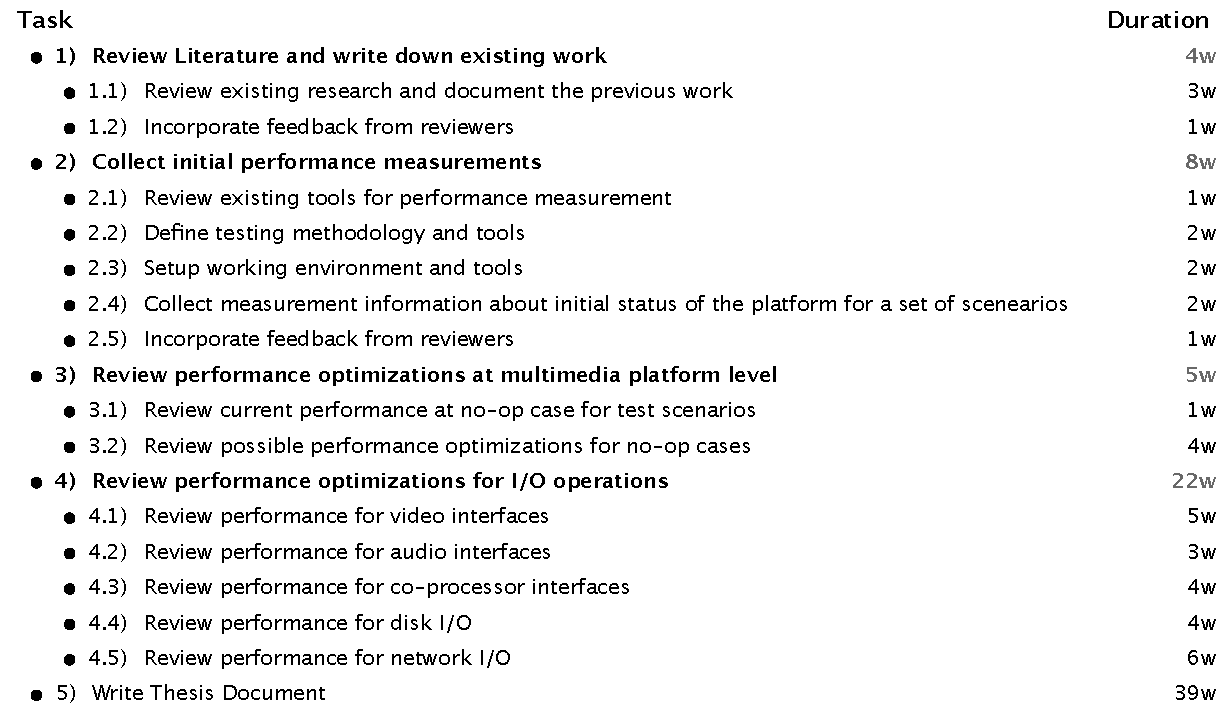
\includegraphics[width=1.0\textwidth]{images/Outline.pdf}
\end{tabular}
\end{table}

\begin{figure}[tbh]
\centering
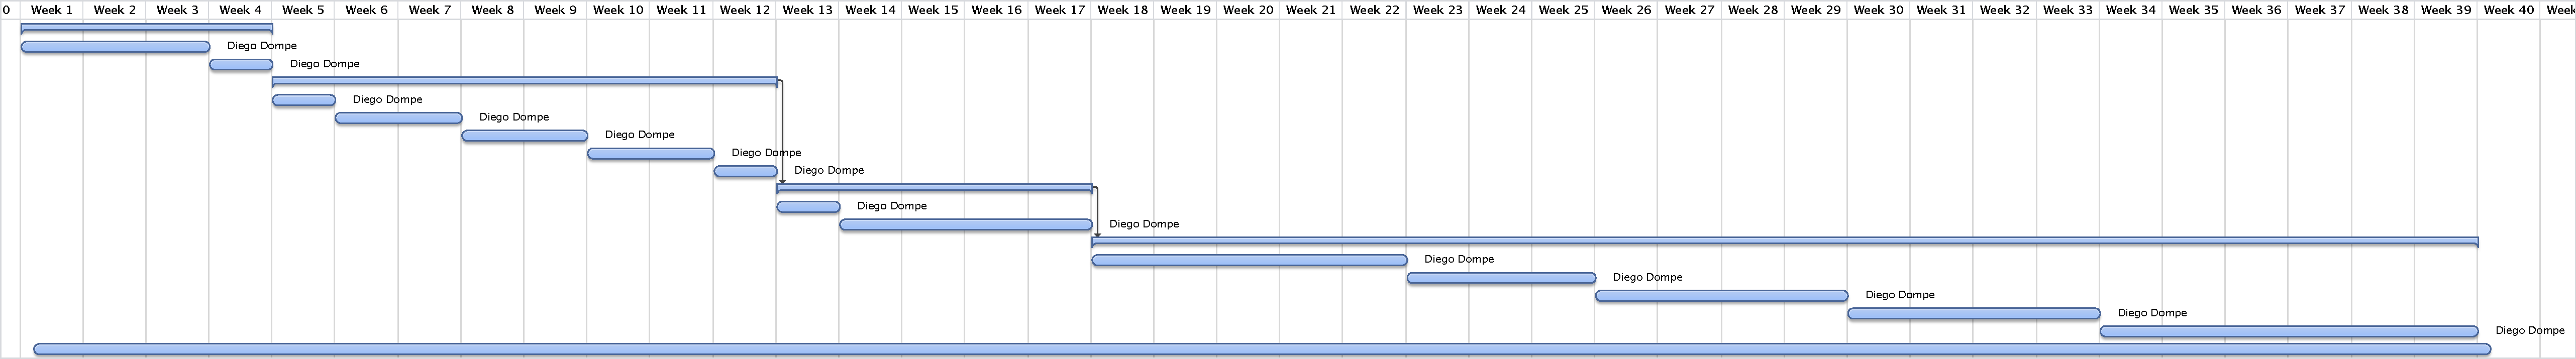
\includegraphics[width=0.85\textheight,angle=90]{images/Gantt.pdf}
\caption{Gantt Chart}\label{gantt}
\end{figure}
